\chapter{Related Work}
\label{chp:b2}

\section{HDR Imaging}

While HDR imaging has long been an active field of research, recent developments in HDR imaging~\cite{Rein2010,Banterle2011,chalmers2016high}, in particular those pertaining to HDR image and video capture~\cite{tocci2011versatile,froehlich2014creating} and display systems~\cite{seetzen2004high}, and HDR
video streaming standards~\cite{standard2016dynamic} to allow direct rendition of HDR images will likely make HDR images more ubiquitous in the near future. However, despite the practical improvements in the field, there is also a need for fundamental and experimental research that explores various aspects related to HDR imaging and dynamic range. Hanhart et al. investigated the performance of various objective metrics in quantifying visual distortions of HDR images commensurate with subjective opinions~\cite{hanhart2015benchmarking}. The authors found HDR-VDP-2~\cite{mantiuk2011hdr} and HDR-VQM~\cite{narwaria2015hdr} to be the best predictors of visual quality. In another study, Grimaldi et al. investigated how image statistics change as a function of dynamic range and found that there are indeed differences between HDR and LDR images~\cite{grimaldi2019statistics}. The authors, also found, however, that the majority of these differences are accounted for by the early visual processing that takes place in the human visual system. However, these works do not consider the HDR image similarity problem.


\subsection{Tone Mapping}
HDR images can capture the true dynamic range of a scene by using wider representations compared to standard 8 bit images. However, in order to display or print HDR images on conventional devices, the dynamic range of the image should be compressed to match the dynamic range of the device. This operation, namely tone mapping, aims to compress the dynamic range while keeping the visual appearance intact. 

Tone mapping is an extensively studied research area and there are many tone mapping operators~\cite{Rein2010}. In this thesis, to investigate the effect of tone mapping operators to visual similarity, eleven commonly used tone mapping operators are selected. Basically, these tone mapping operators can be divided into three categories depending on their operation domain: global and local operators in spatial domain, and gradient domain operators~\cite{Rein2010}. 

Global tone mapping operators apply the same non-linear function to all luminance values without considering pixel neighbourhood. This makes these operators fast compared to other tone mapping operators however, they may result with contrast loss in dark and bright regions. Reinhard et al.~\cite{reinhard2002photographic} introduces a transfer function that compresses low luminance values less and high luminance values more. Drago et al. \cite{drago2003adaptive} uses logarithmic compression for tone mapping while adaptively changing the logarithm base depending on the luminance value. A global algorithm is proposed by Pattanaik et al.~\cite{pattanaik2000time}, which takes in to account the illumination adaptation time of HSV. Other global methods that model photoreceptors of HVS is the work from Reinhard \& Devlin ~\cite{reinhard2005dynamic} and Ferradans et al.~\cite{ferradans2011analysis}. Mantiuk et al. ~\cite{mantiuk2008display} models the display as well as HSV. On the other hand, Mai et al.~\cite{mai2010optimizing} proposed a TMO that minimizes the mean square error between the input HDR and the result of inverse tone mapping.

Local TMOs are computationally more expensive than global TMOs but they may preserve the details better~\cite{Rein2010}. A local TMO that is inspired dodging and burning technique of traditional photography is also given in \cite{reinhard2002photographic}. This operator darkens or brightens the pixel using Gaussian filters on different scales to increase the contrast  depending on the luminance of the pixels in the neighborhood. Another local TMO, proposed by Durand \& Dorsey \cite{durand2002fast}, separated the image to base and detail using bilateral filter and compress only the base level to preserve the details. 

There are also TMOs that operate on gradient domain rather than the spatial domain. Fattal et al.~\cite{fattal2002gradient} suggest to reduce the magnitudes of the high gradients more than the gradients with low magnitude. Then, a low dynamic range image is obtained by solving a Poisson equation on this magnitude-wise altered gradient map. Mantiuk et al.~\cite{mantiuk2006perceptual} follows a similar approach with some improvements on local contrast by using a bigger neighborhood and multi level Gaussian pyramid to enhance global contrast.

In Figure~\ref{fig:tmos}, tone mapping results for the "Belgium House" HDR image is given for several tone mapping operators. fpstools~\cite{HDRGallery} implementation is used for the operators with the default parameters for each operator. As depicted in the figure, tone mapping operators give different results for the same scene in terms of image properties like brightness and color.


\begin{figure}
\begin{subfigure}[b]{0.33\textwidth}
    \centering
    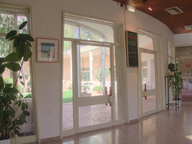
\includegraphics[width=\textwidth]{figures/chapter2/tmos44/44_drago03.png}
    \caption{Drago et al. ~\cite{drago2003adaptive}}
\end{subfigure}\hfill
\begin{subfigure}[b]{0.33\textwidth}
    \centering
    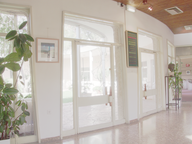
\includegraphics[width=\textwidth]{figures/chapter2/tmos44/44_mai11.png}
    \caption{Mai et al. ~\cite{mai2010optimizing}}
\end{subfigure}\hfill
\begin{subfigure}[b]{0.33\textwidth}
    \centering
    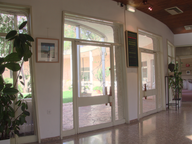
\includegraphics[width=\textwidth]{figures/chapter2/tmos44/44_reinhard02.png}
    \caption{Reinhard et al. (local) ~\cite{reinhard2002photographic}}
\end{subfigure}\\
\begin{subfigure}[b]{0.33\textwidth}
   \centering
    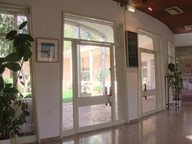
\includegraphics[width=\textwidth]{figures/chapter2/tmos44/44_reinhard02_global.png}
    \caption{Reinhard et al.(global) ~\cite{reinhard2002photographic}}
\end{subfigure}\hfill
\begin{subfigure}[b]{0.33\textwidth}
    \centering
    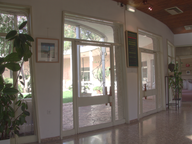
\includegraphics[width=\textwidth]{figures/chapter2/tmos44/44_durand02.png}
    \caption{Durand \& Dorsey~\cite{durand2002fast}}
\end{subfigure}\hfill
\begin{subfigure}[b]{0.33\textwidth}
    \centering
    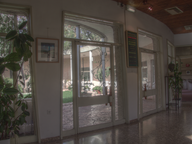
\includegraphics[width=\textwidth]{figures/chapter2/tmos44/44_mantiuk06.png}
    \caption{Mantiuk et al.~\cite{mantiuk2006perceptual}}
\end{subfigure}\\
\begin{subfigure}[b]{0.33\textwidth}
    \centering
    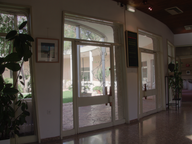
\includegraphics[width=\textwidth]{figures/chapter2/tmos44/44_reinhard05.png}
    \caption{Reinhard \& Devlin~\cite{reinhard2005dynamic}}
\end{subfigure}\hfill
\begin{subfigure}[b]{0.33\textwidth}
    \centering
    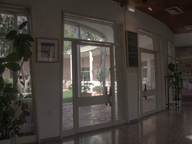
\includegraphics[width=\textwidth]{figures/chapter2/tmos44/44_fattal02.png}
    \caption{Fattal et al.~\cite{durand2002fast}}
\end{subfigure}\hfill
\begin{subfigure}[b]{0.33\textwidth}
    \centering
    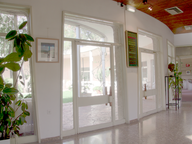
\includegraphics[width=\textwidth]{figures/chapter2/tmos44/44_mantiuk08.png}
    \caption{Mantiuk et al.~\cite{mantiuk2008display}}
\end{subfigure}\hfill\\
\begin{subfigure}[b]{0.33\textwidth}
    \centering
    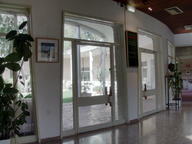
\includegraphics[width=\textwidth]{figures/chapter2/tmos44/44_ferradans11.png}
    \caption{Ferradans et al.~\cite{ferradans2011analysis}}
\end{subfigure}\hspace{-1pt}
\begin{subfigure}[b]{0.33\textwidth}
    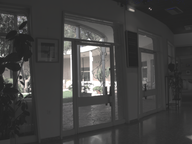
\includegraphics[width=\textwidth]{figures/chapter2/tmos44/44_pattanaik00.png}
    \caption{Pattanaik et al.~\cite{pattanaik2000time}}
\end{subfigure}\hfill
\caption{Tone mapping results for the "Belgium House" HDR image with different tone mapping operators. Note that pfstools~\cite{HDRGallery} implementation is used with default parameters.}
\label{fig:tmos}
\end{figure}

\section{Image Similarity}

Traditionally, image similarity is measured by measuring the distance between hand crafted features extracted from each image. These hand crafted features include simple descriptors such as color/luminance histograms, or improved ideas, including histogram of oriented gradients~\cite{dalal2005histograms}. GIST~\cite{oliva2001modeling}, SIFT~\cite{lowe2004distinctive}, SURF~\cite{bay2006surf}. These features are compared using several types of distance metrics. Recently, deep convolutional neural networks (DCNNs) became the state of art for image classification. Starting with AlexNet~\cite{krizhevsky2012imagenet} and followed by deeper networks such as VGG~\cite{simonyan2014very}, GoogleNet\cite{szegedy2015going}, and ResNet~\cite{he2016deep}, DCNNs started to perform near human level success for image classification. Their success lead to use feature vectors that have been obtained from DCNNs for image retrieval~\cite{wan2014deep,gordo2016deep,noh2017large,radenovic2018fine}. Unlike previous approaches that are based on hand-crafted features, DCNNs learn the feature vector itself directly from the image. 

The similarity between deep learning features can be calculated directly with euclidean or cosine distance without any learning, or can be learned. \cite{frome2007image}, \cite{mcfee2010metric}, \cite{liang2016optimizing} and  OASIS\cite{chechik2010large} are famous similarity learning techniques, that can be classified linear metric learning. These works proposed to work on hand-crafted image features but shown in \cite{wan2014deep} that can also work with deep features. The second group of metric learning is nonlinear metric learning methods, that learn similarity metric directly with deep neural network architectures\cite{pinheiro2018unsupervised}. Siamese\cite{chopra2005learning}\cite{bell2015learning} and triplet\cite{wang2014learning} \cite{arandjelovic2016netvlad} architectures minimizes the classification loss function while a more recent study \cite{garcia2019learning} proposes similarity network architecture to obtain similarity score by minimizing a ranking loss function.

One major drawback of using DCNNs is the need for using very large labeled datasets for training, which is difficult to obtain or not available at all for most problem domains. Transfer learning~\cite{yosinski2014transferable} aims to solve this problem by using pretrained networks on large scale datasets such as ImageNet~\cite{russakovsky2015imagenet}. The basic method is to give the images to the pre-trained network and use the output of the last fully connected layers as feature vectors~\cite{donahue2014decaf,wan2014deep} -- an approach that is also adopted in this thesis.

Visual similarity is a perceptual phenomenon without ground-truth data. This makes collecting data using crowdsourcing experiments valuable. Indeed, there are several crowdsourcing-based works~\cite{lun2015elements,saleh2015learning,kleiman2016toward} that address shape or style similarity problems and conduct user experiments to either derive or validate models. 

Of most related to our work are two similarity studies that also employ subjective experiments. Among these, in Rogowitz et al.~\cite{rogowitz1998perceptual}, human participants are asked to judge image similarity using two different experiments: one involving printouts of images (called table scaling) and the other using a computer based comparison (called computer scaling). These results are compared with computational similarity approaches~\cite{frese1997methodology} and simple CIELAB histograms. It was found that both table and computer scaling yield similar results and color is a major factor influencing similarity for human observers.

In another study~\cite{neumann2006image}, user experiments are conducted to evaluate the relationship between an image-indexing system and perceived similarity in an LDR setting. The tested image indexing system is based on basic properties of early stages of human vision -- chromaticity, luminance, and texture. Two-alternative forced-choice (2AFC) method is used for all experiments. Three images are shown to the observer, the query image and two test images. Of these two images one image is called the target and the other the distractor. These images are selected based on the rankings obtained from the image-indexing system. Then the correlation between the users' preference and index rank is investigated. First, each index, chromaticity, luminance, and texture are calculated separately. From these indexes chromaticity is found to give the best results. Then for the second experiment, combinations of the indexes are evaluated. The combination of chromaticity and texture indices are found to give better results than chromaticity alone and the combination of all indices are found to give the best result.

As mentioned above, although visual image similarity is an extensively studied subject~\cite{liu2007survey}, to our knowledge there is no study that directly addresses this problem for HDR images. Thus, understanding the nature of image similarity for HDR images and developing an objective similarity measure is the primary goal of this thesis. 

\section{Image Features}
\label{sec:features}
As the most fundamental part of many computer vision applications, image feature extraction is a widely studied research topic for the last several decades. There are numerous image features in the literature developed with different purposes which can be divided into two broad categories: global and local features. While global features like histograms of image properties represent the whole image with a single feature vector, local features like SIFT~\cite{lowe2004distinctive} or SURF~\cite{bay2006surf} are a collection of vectors representing small neighborhoods called interest regions. Although local features are used successfully for the applications like image classification or retrieval, this thesis focuses on global features to investigate the image similarity in a general sense. In this section, a review of global image features that have been used in this thesis is given. Table~\ref{tab:table_feature} lists these features together with their representations and the distance metric used for each feature. 

\begin{table}
\caption{HDR Image features and distances}
\centering
\begin{tabular}{c|c|c}
\label{tab:table_feature}
\textbf{Feature} & \textbf{Model} & \textbf{Distance Metric}\\
\hline
Color  & 2D chromaticity histogram & EMD \\
Luminance  & 1D (relative) luminance histogram & EMD \\
Texture  & Histograms of gradients & EMD \\
GIST  & Feature vector & Cosine distance \\
VGG16/VGG19 - fc6 & Fused fc6 layer & Cosine distance  \\
VGG16/VGG19 - fc7 & Fused fc7 layer & Cosine distance
\end{tabular}
\end{table}

%paper
\subsection{Color}
%paper
Since the early days of the image similarity research, color has been used as one of the most discriminative cues~\cite{neumann2006image}. In this thesis,  we used the $a$ and $b$ channels of the CIELAB color space~\cite{iso201111664} to represent chromaticity information. This is an opponent color space, where the $a$ channel represents red/green opponent colors and the $b$ channel yellow/blue opponent colors. We used a 2D chromaticity histogram to represent the distribution of colors in a given image. Each dimension contained $15$ bins for a total of $225$ bins. Figure~\ref{fig:hists} shows this histogram for the Mason Lake image from the dataset~\cite{fairchild2007hdr}.

\begin{figure}
\centering
\begin{tabular}{c c}
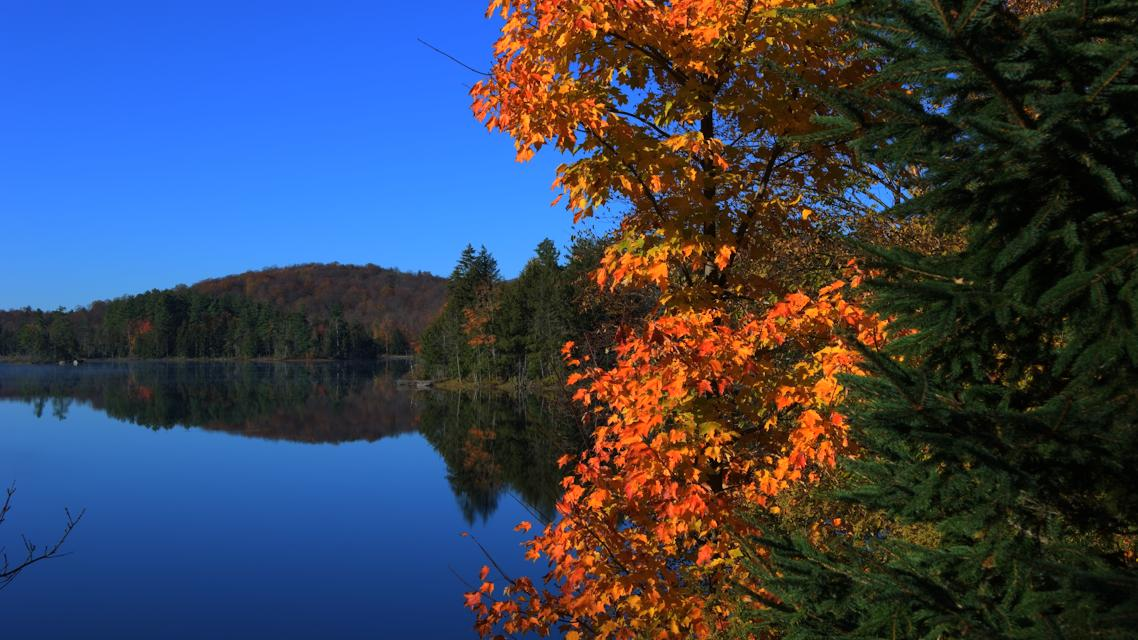
\includegraphics[height=1.8in]{figures/chapter2/MasonLake.jpg} &
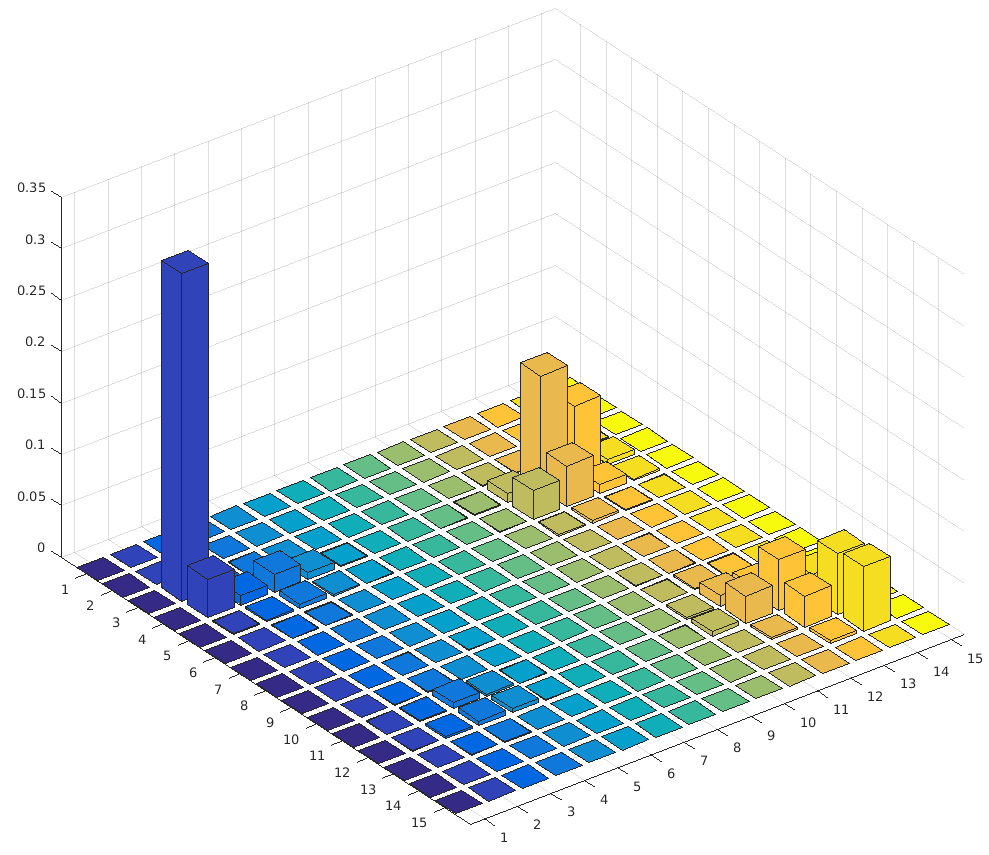
\includegraphics[height=1.8in]{figures/chapter2/57_histab.png}
\end{tabular}
\caption{Sample image (left), 2D histogram (right).}
\label{fig:hists}
\end{figure}

%paper
\subsection{Texture}
%paper
Texture is the second most used feature for content based image retrieval systems after chromatic features. This feature is especially helpful for discriminating images that have similar color but different spatial characteristics such as blue sky and sea or sand and buildings. In this thesis, to represent the texture information histogram of gradient magnitudes~\cite{sharma2015histogram} is used. 
%paper
\subsection{Luminance}
%paper
The main difference between an HDR and an LDR image is the much wider range of luminance distribution for the former. A single HDR image may contain very low luminances corresponding to highly shadowed regions as well as very high luminances corresponding to bright highlights. Therefore, we hypothesized that the luminance distribution of an HDR image may be an important cue for visual similarity. The luminance distribution is modeled using a 1D (relative) luminance histogram with $50$ bins.
%paper
\subsection{GIST Features}
%paper
The GIST descriptor~\cite{oliva2001modeling} aims to represent the dominant spatial structure of a scene by using low level multi-scale representations. This descriptor defines the scene as a whole rather than focusing on individual objects or regions. Discriminative properties of a scene are listed as naturalness, openness, roughness, expansion, and ruggedness. The class of a scene, e.g., man-made, natural, indoor, outdoor, etc., is determined by these properties.

The procedure for extracting GIST descriptors consists of applying Gabor filters that are scaled and orientated differently to the input image, dividing the filter response map into a grid in order to have spatial information, averaging the filter response in each grid, and concatenating the results to obtain the final feature vector, i.e. the GIST descriptor.

%paper
\subsection{Deeply Learned Features}
%paper
Recently, DCNNs have started to dominate object recognition and image classification tasks, achieving near human success rates~\cite{krizhevsky2012imagenet,simonyan2014very,zhou2017scene}. These models are trained with large prelabeled datasets and develop a hierarchical model that becomes more aware of the content of the image rather than the underlying pixel values. To our knowledge currently there is no DCNN model that is trained on HDR images for the purpose of image indexing, scene classification, or visual similarity tasks.
Furthermore, there is no prelabeled large HDR image dataset to use for training a DCNN model from scratch. Therefore in this thesis, we used transfer learning method to employ pretrained DCNNs for our perceptual similarity problem. 

For feature extraction, pretrained AlexNet~\cite{krizhevsky2012imagenet} and two variants of VGG networks, VGG16 and VGG19, are used~\cite{simonyan2014very}. All networks are trained on the ImageNet~\cite{russakovsky2015imagenet} dataset, but we also evaluated their performance when trained using different datasets. For transfer learning, the last fully connected layer, which contains classification outputs, is removed and the remaining $4096$ dimensional two fully connected layers, \textbf{fc6} and \textbf{fc7}, are used as feature vectors. As suggested by Simonyan and Zisserman~\cite{simonyan2014very}, the results obtained from VGG16 and VGG19 are fused (by taking an average) and it is observed that the fused version performs better than both VGG16 and VGG19. The distance between the feature vectors are calculated using cosine distance, which is a commonly used distance metric for deep learning features. 

%\section{Computational Complexity}
%As attentive readers may inquire about the computational complexity of these features, a brief analysis is provided in this section. The color and luminance features are merely histograms and they can be computed in O(N) time, where N represents the number of image pixels. The GIST descriptor is based on computing the convolution of 32 Gabor filters at 4 scales and 8 orientations to compute feature maps and then averaging the features to obtain a 16 element vector per feature map. These vectors are then concatenated to find the final feature vector. Therefore, the GIST feature also has a linear time computational complexity. The texture feature represented by HOG is similar to GIST in terms of its operation, albeit being somewhat simpler, and also has a linear complexity. Finally, the deeply learned features are computed by a single forward application of the VGG network, which also involves several convolutions at multiple scales as well as application of activation functions. As the convolutional kernel sizes are negligible compared to the image size, the computation of VGG features also has a linear time computational complexity. In summary, all of the features can be computed at real-time rates in modern hardware, especially if GPUs are utilized.
%paper
\section{Distance Metrics}
%paper
The use of a proper distance metric is as important as the features themselves. Each feature representation
may require a different distance metric. In this section, we briefly describe the definitions and properties of the dissimilarity measures that we used for different types of features.
%paper
\subsection{Euclidean Distance}
%paper
The Euclidean distance between two histograms p and q is calculated as:
\begin{equation}
dist_{euc}(p,q) = \sqrt{\sum_i(p_i-q_i)^2},
\end{equation}
where i is the bin index. In general, dissimilarity obtained by Euclidean distance for histograms is not satisfactory as it does not take bin proximity into account.
%paper
\subsection{Bhattacharyya Distance}
%paper
Bhattacharyya distance~\cite{bhattacharyya1946measure} measures the overlap between two distributions. If p and q are two histograms, it can be calculated as:
\begin{equation}
dist_{bhat}(p,q) = -\ln \left( \sum_i \sqrt{p_i.q_i} \right).
\end{equation}

For our HDR similarity problem Bhattacharyya distance gives slightly better results than Euclidean distance. However, it also suffers from the same problem that the proximity of the bins is not taken into account.
%paper
\subsection{Earth Mover’s Distance}
%paper
Earth Mover’s Distance (EMD) is a dissimilarity metric commonly used for image the retrieval problems~\cite{rubner2000earth}. EMD aims to capture the perceptual similarity between two distributions by calculating the minimal cost of transforming one distribution to the other. Unlike the other dissimilarity metrics, EMD can be calculated for varying-size partitions of the data, called signatures.
Signatures consist of dominant clusters of the data, represented as $si = (m_i, w_i)$ pairs where mi is the cluster center and $w_i$ is the size of the cluster. EMD does not require the signatures to have the same number of clusters – ground distances between cluster centers are sufficient. Histograms are signatures with bin centers corresponding to cluster centers, mi, and normalized bin values to weights, $w_i$.

The total amount of work to transform distribution
p to q with flow f is:
\begin{equation}
WORK(P,Q,F) = \sum_i^m \sum_j^n d_{ij}f_{ij}, 
\end{equation}
where dij is the ground distance between cluster centers i and j. The optimal flow f that results with the minimum work, can be found by any linear optimization algorithm. When f is calculated, the EMD between p and q is defined as:
\begin{equation}
EMD(p,q) = {{\sum \sum d_{ij}f_{ij}}\over{\sum \sum f_{ij}}}.
\end{equation}
In our problem, bin centers correspond to color values (ab values in the CIELAB space) and ground distances are calculated as Euclidean because of the perceptual uniformity of the CIELAB color space.

Figure \ref{fig:sim_comp} compares the effect of these three distance metrics for a sample image from the dataset. The image on the first column is the query image, and in each row, the most similar five images from the dataset are shown. The distance metric used in first row is Euclidean, the second row is Bhattacharyya, and the last row is the EMD. It can be argued that more similar images are found using the EMD metric.

\begin{figure} 
\centering
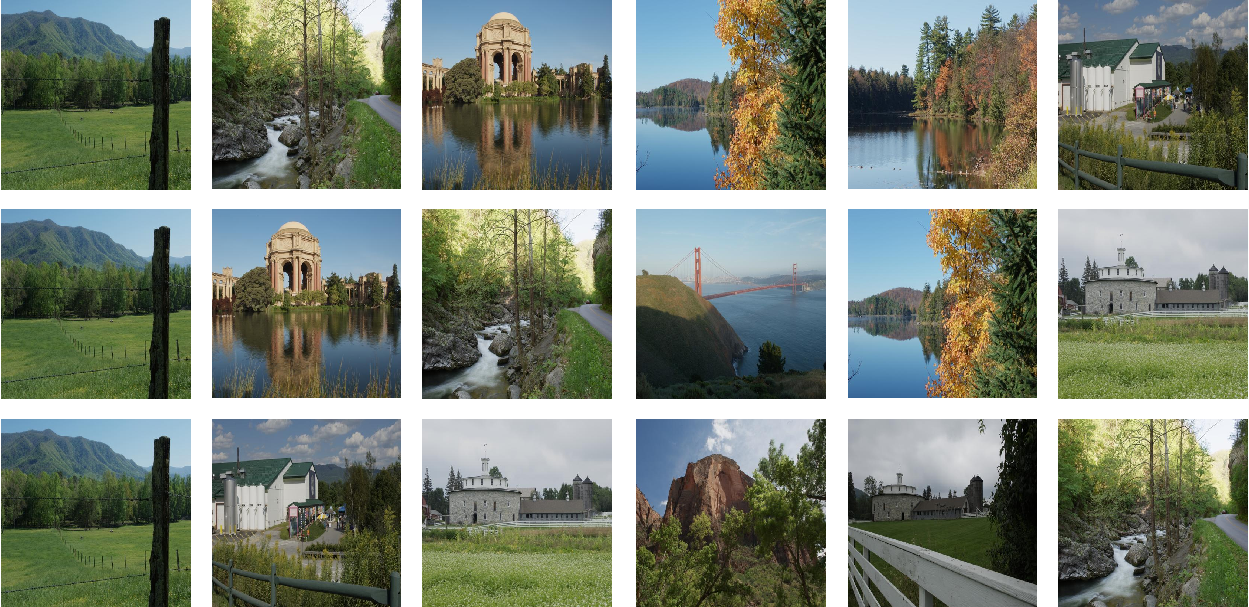
\includegraphics[width=\textwidth]{figures/chapter2/16sims.png}
\vspace{10pt}
\caption{A comparison of dissimilarity metrics for histogram-based features. The leftmost image is the query image, the most similar five images from the dataset are shown in each row: Euclidean distance (first row), Bhattacharyya distance (second row), Earth Mover’s distance (third row).}
\label{fig:sim_comp}
\end{figure}

%paper
\subsection{Cosine Similarity}
%paper
Cosine distance between two vectors $p$ and $q$ is calculated as:
\begin{equation}
dist_{cosine}(p,q) = 1 - {{\sum_{i=1}^{n}p_{i}q_{i}} \over {\sqrt{\sum_{i=1}^{n}p_{i}^2}} \sqrt{\sum_{i=1}^{n}q_{i}^2}} 
\end{equation}
Cosine distance is a widely used distance metric for deep representations. In this thesis, we used cosine distance for calculating the distances between CNN feature vectors and GIST features.